% Options for packages loaded elsewhere
\PassOptionsToPackage{unicode}{hyperref}
\PassOptionsToPackage{hyphens}{url}
%
\documentclass[
]{article}
\usepackage{lmodern}
\usepackage{amssymb,amsmath}
\usepackage{ifxetex,ifluatex}
\ifnum 0\ifxetex 1\fi\ifluatex 1\fi=0 % if pdftex
  \usepackage[T1]{fontenc}
  \usepackage[utf8]{inputenc}
  \usepackage{textcomp} % provide euro and other symbols
\else % if luatex or xetex
  \usepackage{unicode-math}
  \defaultfontfeatures{Scale=MatchLowercase}
  \defaultfontfeatures[\rmfamily]{Ligatures=TeX,Scale=1}
\fi
% Use upquote if available, for straight quotes in verbatim environments
\IfFileExists{upquote.sty}{\usepackage{upquote}}{}
\IfFileExists{microtype.sty}{% use microtype if available
  \usepackage[]{microtype}
  \UseMicrotypeSet[protrusion]{basicmath} % disable protrusion for tt fonts
}{}
\makeatletter
\@ifundefined{KOMAClassName}{% if non-KOMA class
  \IfFileExists{parskip.sty}{%
    \usepackage{parskip}
  }{% else
    \setlength{\parindent}{0pt}
    \setlength{\parskip}{6pt plus 2pt minus 1pt}}
}{% if KOMA class
  \KOMAoptions{parskip=half}}
\makeatother
\usepackage{xcolor}
\IfFileExists{xurl.sty}{\usepackage{xurl}}{} % add URL line breaks if available
\IfFileExists{bookmark.sty}{\usepackage{bookmark}}{\usepackage{hyperref}}
\hypersetup{
  pdftitle={README},
  hidelinks,
  pdfcreator={LaTeX via pandoc}}
\urlstyle{same} % disable monospaced font for URLs
\usepackage{longtable,booktabs}
% Correct order of tables after \paragraph or \subparagraph
\usepackage{etoolbox}
\makeatletter
\patchcmd\longtable{\par}{\if@noskipsec\mbox{}\fi\par}{}{}
\makeatother
% Allow footnotes in longtable head/foot
\IfFileExists{footnotehyper.sty}{\usepackage{footnotehyper}}{\usepackage{footnote}}
\makesavenoteenv{longtable}
\usepackage{graphicx}
\makeatletter
\def\maxwidth{\ifdim\Gin@nat@width>\linewidth\linewidth\else\Gin@nat@width\fi}
\def\maxheight{\ifdim\Gin@nat@height>\textheight\textheight\else\Gin@nat@height\fi}
\makeatother
% Scale images if necessary, so that they will not overflow the page
% margins by default, and it is still possible to overwrite the defaults
% using explicit options in \includegraphics[width, height, ...]{}
\setkeys{Gin}{width=\maxwidth,height=\maxheight,keepaspectratio}
% Set default figure placement to htbp
\makeatletter
\def\fps@figure{htbp}
\makeatother
\setlength{\emergencystretch}{3em} % prevent overfull lines
\providecommand{\tightlist}{%
  \setlength{\itemsep}{0pt}\setlength{\parskip}{0pt}}
\setcounter{secnumdepth}{-\maxdimen} % remove section numbering
\ifluatex
  \usepackage{selnolig}  % disable illegal ligatures
\fi

\title{README}
\author{}
\date{}

\begin{document}
\maketitle

\hypertarget{binary-heap-implementation---array-based-implementation}{%
\subsection{Binary Heap Implementation - Array Based
Implementation}\label{binary-heap-implementation---array-based-implementation}}

\hypertarget{needs-some-tweeking}{%
\subsubsection{NEEDS SOME TWEEKING}\label{needs-some-tweeking}}

In this Heap overview, we assume \textbf{MIN} heap.

\hypertarget{overview}{%
\subsubsection{Overview}\label{overview}}

In order to make our heap work efficiently, we will take advantage of
the logarithmic nature of the binary tree to represent our heap. In
order to guarantee logarithmic performance, we must keep our tree
balanced. A balanced binary tree has roughly the same number of nodes in
the left and right subtrees of the root. In our heap implementation we
keep the tree balanced by creating a \textbf{complete binary tree}. A
complete binary tree is a tree in which each level has all of its nodes.
The exception to this is the bottom level of the tree, which we fill in
from left to right. The Figure below shows an example of a complete
binary tree.

\begin{longtable}[]{@{}c@{}}
\toprule
A Complete Binary Tree\tabularnewline
\midrule
\endhead
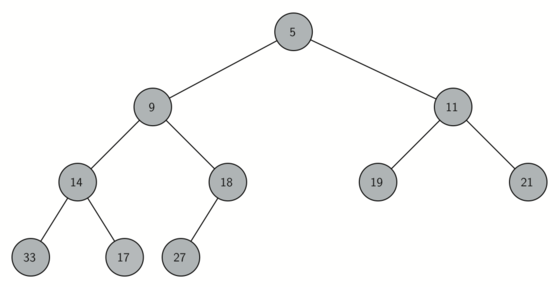
\includegraphics{https://cs.msutexas.edu/~griffin/zcloud/zcloud-files/compTree_3013_2020.png}\tabularnewline
\bottomrule
\end{longtable}

\begin{itemize}
\tightlist
\item
  Another interesting property of a complete tree is that we can
  represent it using a single list. We do not need to use nodes and
  references or even lists of lists.
\item
  Because the tree is complete, the left child of a parent (at position
  \emph{P}) is the node that is found in position \textbf{\emph{2P}} in
  the list.
\item
  Similarly, the right child of the parent is at position
  \textbf{\emph{2P + 1}} in the list.
\item
  To find the parent of any node in the tree, we can simply use C++'s
  integer division. Given that a node is at position \textbf{\emph{n}}
  in the list, the parent is at position \textbf{\emph{n/2}}.
\item
  The figure below shows a complete binary tree and also gives the list
  representation of the tree.
\item
  Note the \textbf{\emph{2P}} and \textbf{\emph{2P + 1}} relationship
  between parent and children.
\item
  The list representation of the tree, along with the full structure
  property, allows us to efficiently traverse a complete binary tree
  using only a few simple mathematical operations. We will see that this
  also leads to an efficient implementation of our binary heap.
\end{itemize}

\begin{longtable}[]{@{}c@{}}
\toprule
A Complete Binary Tree w/ List Representation\tabularnewline
\midrule
\endhead
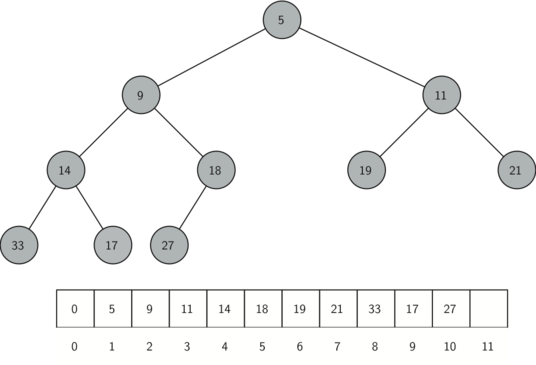
\includegraphics{https://cs.msutexas.edu/~griffin/zcloud/zcloud-files/heapOrder_3013_2020.png}\tabularnewline
\bottomrule
\end{longtable}

\hypertarget{the-heap-order-property}{%
\subsection{The Heap Order Property}\label{the-heap-order-property}}

\begin{itemize}
\tightlist
\item
  The method that we will use to store items in a heap relies on
  maintaining the heap order property.
\item
  The \textbf{heap order property} is as follows: \textgreater{} In a
  heap, for every node \textbf{\emph{x}} with parent \textbf{\emph{p}},
  the key in \textbf{\emph{p}} is smaller than or equal to the key in
  \textbf{\emph{x}}.
\end{itemize}

\hypertarget{heap-operations}{%
\subsection{Heap Operations}\label{heap-operations}}

\hypertarget{getting-setup}{%
\subsubsection{Getting Setup}\label{getting-setup}}

Since the entire binary heap can be represented by a single array
(efficiently), we don't need to keep track of much. Remember that since
a heap is ALWAYS a complete tree, we never have empty slots between
stored values in our array. We really only need to keep track of the
\textbf{\emph{next available slot}} (or \textbf{\emph{currentSize}}).

Also, we start filling our array at \textbf{\emph{index 1}} since using
\textbf{\emph{index 0}} would have bad results when calculating
\emph{left, right, and parent.} The figure below shows the relationship
between each binary tree entity when stored in an array.

\begin{longtable}[]{@{}c@{}}
\toprule
Heap Container\tabularnewline
\midrule
\endhead
\textbf{Empty Container - We don't use slot zero.}\tabularnewline
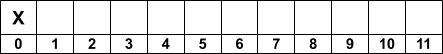
\includegraphics{https://cs.msutexas.edu/~griffin/zcloud/zcloud-files/3013.heap_array_2020.png}\tabularnewline
\textbf{\emph{Parent Vs Left and Right Child}}\tabularnewline
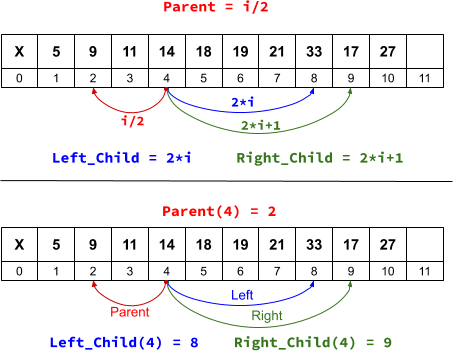
\includegraphics{https://cs.msutexas.edu/~griffin/zcloud/zcloud-files/3013_heap_array_2c_2020.png}\tabularnewline
\bottomrule
\end{longtable}

\hypertarget{insert}{%
\subsubsection{Insert}\label{insert}}

The easiest, and most efficient, way to add an item to a heap is to
simply append the item to the next available slot in the array. The good
news about this is that we will ALWAYS have a complete tree! The bad
news about appending is that we will very likely violate the heap
structure property (meaning we will have to re-arrange values).

Fixing any violations of the heap structure property can be done by
comparing the newly added item with its parent. If the newly added item
is less than its parent, then we can swap the item with its parent. The
figure below shows the series of swaps needed to percolate the newly
added item up to its proper position in the tree.

\begin{longtable}[]{@{}cc@{}}
\toprule
Binary Tree (What we picture) & Array (Whats really
happening)\tabularnewline
\midrule
\endhead
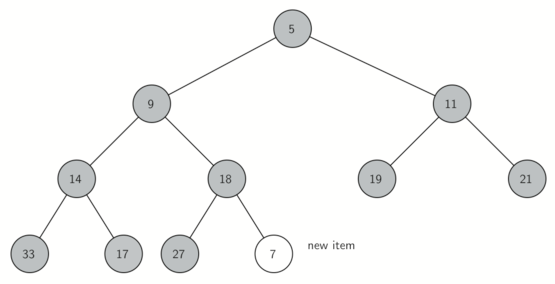
\includegraphics[width=3.125in,height=\textheight]{https://cs.msutexas.edu/~griffin/zcloud/zcloud-files/3013_heap_percup_1.png}
&
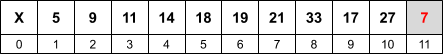
\includegraphics[width=0.75\textwidth,height=\textheight]{https://cs.msutexas.edu/~griffin/zcloud/zcloud-files/3013_heap_insert_1_2020.png}\tabularnewline
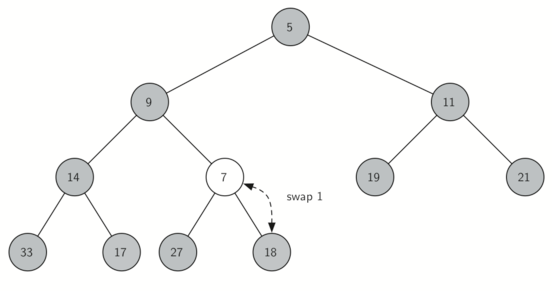
\includegraphics[width=3.125in,height=\textheight]{https://cs.msutexas.edu/~griffin/zcloud/zcloud-files/3013_heap_percup_2.png}
&
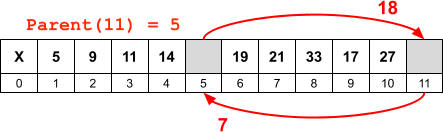
\includegraphics[width=0.75\textwidth,height=\textheight]{https://cs.msutexas.edu/~griffin/zcloud/zcloud-files/3013_heap_insert_2_2020.png}\tabularnewline
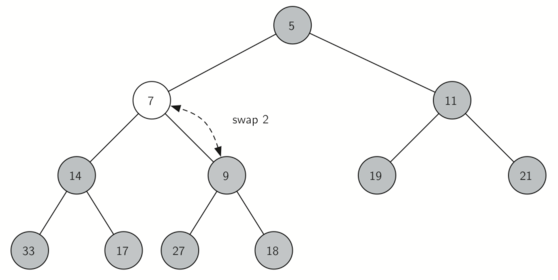
\includegraphics[width=3.125in,height=\textheight]{https://cs.msutexas.edu/~griffin/zcloud/zcloud-files/3013_heap_percup_3.png}
&
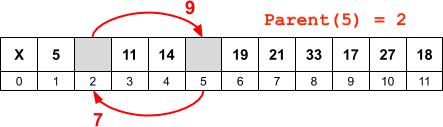
\includegraphics[width=0.75\textwidth,height=\textheight]{https://cs.msutexas.edu/~griffin/zcloud/zcloud-files/3013_heap_insert_3_2020.png}\tabularnewline
\bottomrule
\end{longtable}

Notice that when we percolate an item up, we are restoring the heap
property between the newly added item and the parent. We are also
preserving the heap property for any siblings. Of course, if the newly
added item is very small, we may still need to swap it up another level.
In fact, we may need to keep swapping until we get to the top of the
tree. The figure above shows the \texttt{percUp} or \texttt{bubbleUp}
method, which percolates a new item as far up in the tree as it needs to
go to maintain the heap property. Again, we use \textbf{\emph{i / 2}} to
find the parent and swap the values if the child is smaller than the
parent.

\hypertarget{removemin}{%
\subsubsection{RemoveMin}\label{removemin}}

Since the heap property requires that the root of the tree be the
smallest item in the tree, finding the minimum item is easy. The hard
part of \texttt{RemoveMin} is restoring full compliance with the heap
structure and heap order properties after the root has been removed. We
can restore our heap in two steps.

\begin{enumerate}
\def\labelenumi{\arabic{enumi}.}
\tightlist
\item
  First, we will restore the root item by taking the last item in the
  list and moving it to the root position. Moving the last item
  maintains our heap structure property. However, we have probably
  destroyed the heap order property of our binary heap.
\item
  Second, we will restore the heap order property by pushing the new
  root node down the tree to its proper position. The figure below shows
  the series of swaps needed to move the new root node to its proper
  position in the heap.
\end{enumerate}

\begin{longtable}[]{@{}cc@{}}
\toprule
Binary Tree (What we picture) & Array (Whats really
happening)\tabularnewline
\midrule
\endhead
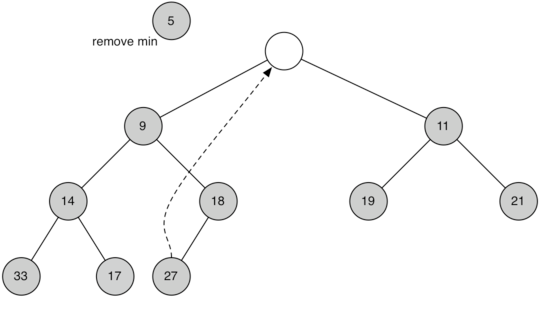
\includegraphics[width=3.125in,height=\textheight]{https://cs.msutexas.edu/~griffin/zcloud/zcloud-files/3013_heap_percdown_1.png}
&
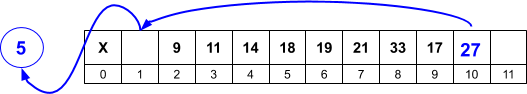
\includegraphics[width=0.75\textwidth,height=\textheight]{https://cs.msutexas.edu/~griffin/zcloud/zcloud-files/3013_heap_percdown_1_array.png}\tabularnewline
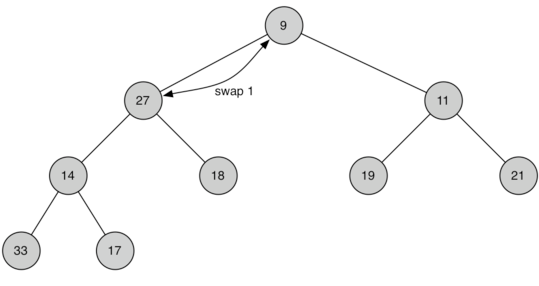
\includegraphics[width=3.125in,height=\textheight]{https://cs.msutexas.edu/~griffin/zcloud/zcloud-files/3013_heap_percdown_2.png}
&
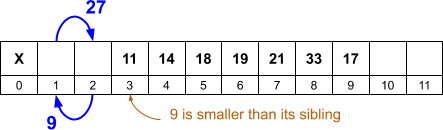
\includegraphics[width=0.75\textwidth,height=\textheight]{https://cs.msutexas.edu/~griffin/zcloud/zcloud-files/3013_heap_percdown_2_array.png}\tabularnewline
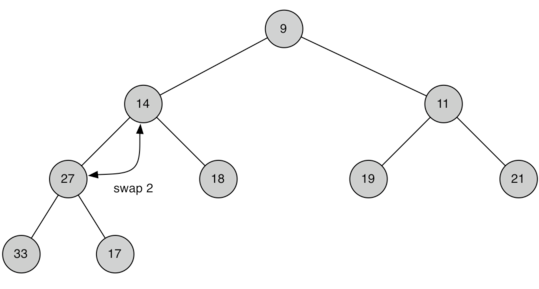
\includegraphics[width=3.125in,height=\textheight]{https://cs.msutexas.edu/~griffin/zcloud/zcloud-files/3013_heap_percdown_3.png}
&
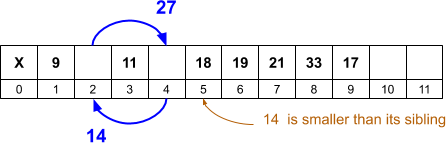
\includegraphics[width=0.75\textwidth,height=\textheight]{https://cs.msutexas.edu/~griffin/zcloud/zcloud-files/3013_heap_percdown_3_array.png}\tabularnewline
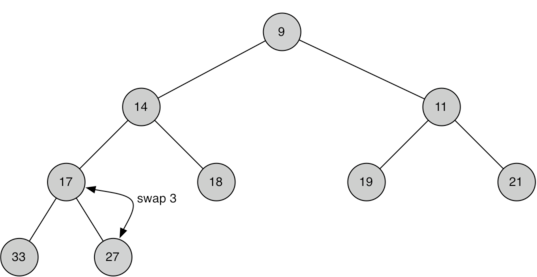
\includegraphics[width=3.125in,height=\textheight]{https://cs.msutexas.edu/~griffin/zcloud/zcloud-files/3013_heap_percdown_4.png}
&
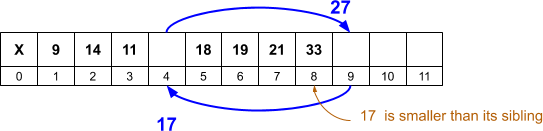
\includegraphics[width=0.75\textwidth,height=\textheight]{https://cs.msutexas.edu/~griffin/zcloud/zcloud-files/3013_heap_percdown_4_array.png}\tabularnewline
\bottomrule
\end{longtable}

In order to maintain the heap order property, all we need to do is swap
the root with its smallest child less than the root. After the initial
swap, we may repeat the swapping process with a node and its children
until the node is swapped into a position on the tree where it is
already less than both children.

\hypertarget{heapify}{%
\subsubsection{Heapify}\label{heapify}}

To finish our discussion of binary heaps, we will look at a method to
build an entire heap from a list of keys. The first method you might
think of may be like the following. Given a list of keys, you could
easily build a heap by inserting each key one at a time. Since you are
starting with a list of one item, the list is sorted and you could use
binary search to find the right position to insert the next key at a
cost of approximately \textbf{\emph{O(lg n)}} operations. However,
remember that inserting an item in the middle of the list may require
\textbf{\emph{O(n)}} operations to shift the rest of the list over to
make room for the new key. Therefore, to insert \textbf{\emph{n}} keys
into the heap would require a total of \textbf{\emph{O(n lg n)}}
operations. However, if we start with an entire list then we can build
the whole heap in \textbf{\emph{O(n)}} operations.

\begin{longtable}[]{@{}cc@{}}
\toprule
Heapify &\tabularnewline
\midrule
\endhead
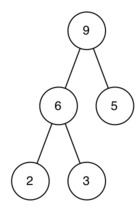
\includegraphics{https://cs.msutexas.edu/~griffin/zcloud/zcloud-files/3013_heapify_tree_1.png}
&
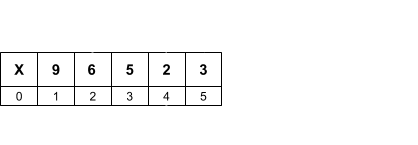
\includegraphics{https://cs.msutexas.edu/~griffin/zcloud/zcloud-files/3013_heapify_array_1.png}\tabularnewline
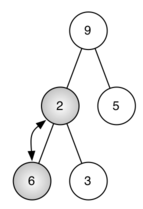
\includegraphics{https://cs.msutexas.edu/~griffin/zcloud/zcloud-files/3013_heapify_tree_2.png}
&
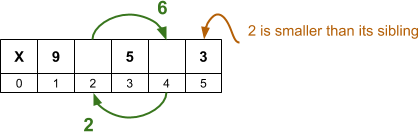
\includegraphics{https://cs.msutexas.edu/~griffin/zcloud/zcloud-files/3013_heapify_array_2.png}\tabularnewline
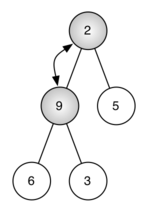
\includegraphics{https://cs.msutexas.edu/~griffin/zcloud/zcloud-files/3013_heapify_tree_3.png}
&
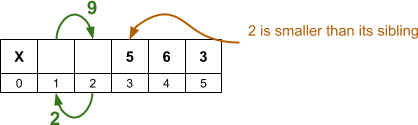
\includegraphics{https://cs.msutexas.edu/~griffin/zcloud/zcloud-files/3013_heapify_array_3.png}\tabularnewline
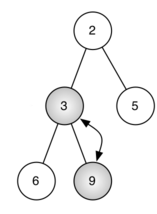
\includegraphics{https://cs.msutexas.edu/~griffin/zcloud/zcloud-files/3013_heapify_tree_4.png}
&
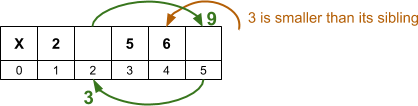
\includegraphics{https://cs.msutexas.edu/~griffin/zcloud/zcloud-files/3013_heapify_array_4.png}\tabularnewline
\bottomrule
\end{longtable}

The figure above shows the swaps that the \texttt{Heapify} method makes
as it moves the nodes in an initial tree of {[}9, 6, 5, 2, 3{]} into
their proper positions. Although we start out in the middle of the tree
and work our way back toward the root, the \texttt{percDown} method
ensures that the largest child is always moved down the tree. Because
the heap is a complete binary tree, any nodes past the halfway point
will be leaves and therefore have no children. Notice that when
\texttt{i=1}, we are percolating down from the root of the tree, so this
may require multiple swaps. As you can see in the bottom most two trees
in the figure above, first the 9 is moved out of the root position, but
after 9 is moved down one level in the tree, \texttt{percDown} ensures
that we check the next set of children farther down in the tree to
ensure that it is pushed as low as it can go. In this case it results in
a second swap with 3. Now that 9 has been moved to the lowest level of
the tree, no further swapping can be done.

The assertion that we can build the heap in \textbf{\emph{O(n)}} may
seem a bit mysterious at first, and were not proving anything. However,
the key to understanding that you can build the heap in
\textbf{\emph{O(n)}} is to remember that the \textbf{\emph{O(lg n)}}
factor is derived from the height of the tree. For most of the work in
\texttt{Heapify}, the tree is shorter than \textbf{\emph{lg n}}.

Using the fact that you can build a heap from a list in
\textbf{\emph{O(n)}} time, you could easily construct a sorting
algorithm that uses a heap and sorts a list in \textbf{\emph{O(n lg n)}}
cost.

\end{document}
